\section{Introduction}
\label{sec:introduction}

Every design decision in software engineering is a compromise with unknown future requirements. A code search program built around regular expressions works until the specification demands structural pattern matching, at which point the entire architecture must be rewritten. Existing coding-agent benchmarks systematically undermeasure this failure mode, evaluating models once against complete task specifications~\citep{swe-bench,projdevbench,vibe-code-bench,swe-rebench-v2}. They measure whether an agent can produce correct code for the current specification, not whether that code remains extensible under future change.

\begin{figure}[t]
    \centering
    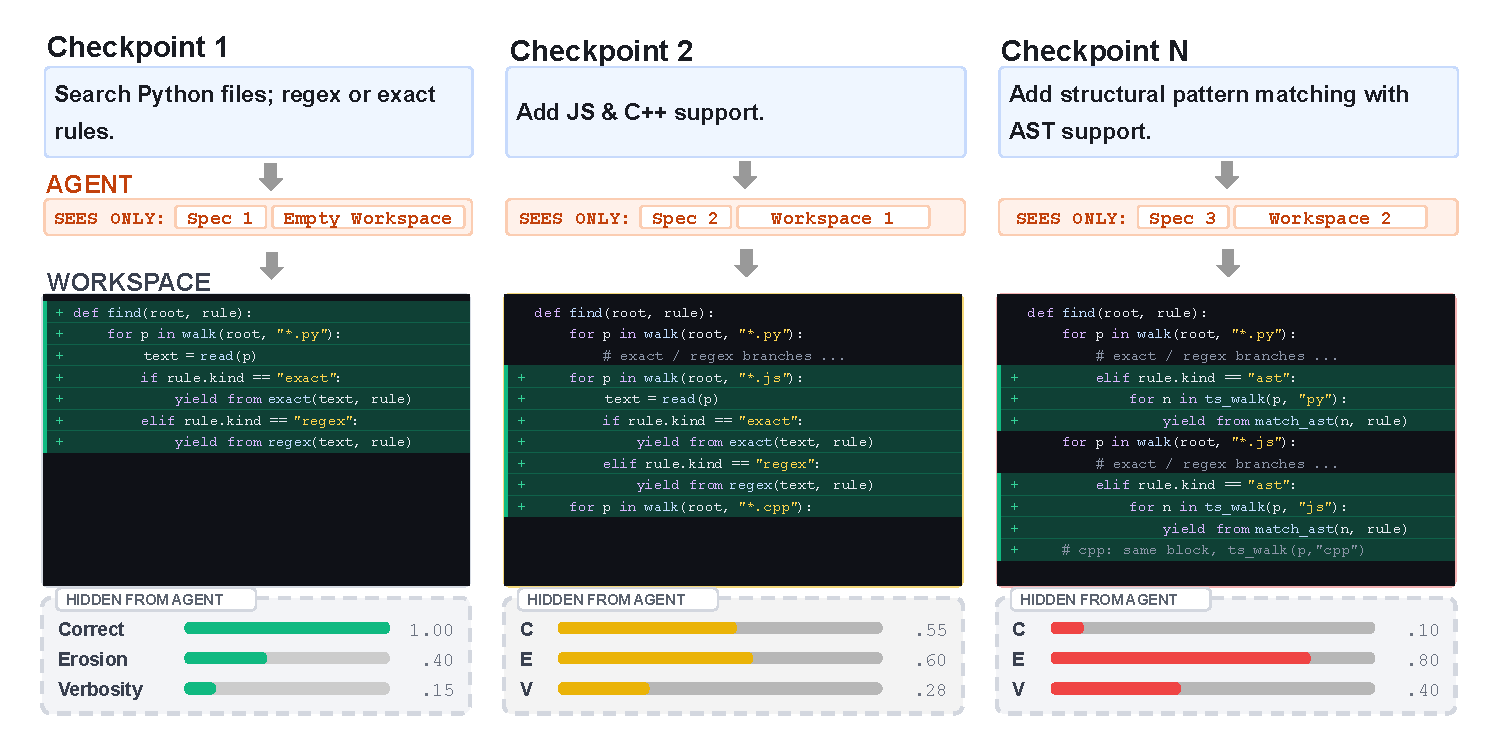
\includegraphics[width=1.00\textwidth]{figures/hero_v3.pdf}
    \caption{\textbf{Iterative evaluation in SCBench.} A task unfolds over checkpoints. 
At each step, the agent extends its prior workspace to satisfy an updated 
spec (orange). Correctness, erosion, and verbosity are scored externally 
and withheld from the agent (gray). Local shortcuts compound: correctness 
falls from $1.00$ to $0.10$ while erosion and verbosity grow.}
    \label{fig:overview}
\end{figure}

Under repeated editing, agent-generated code often deteriorates in recognizable ways. LLMs favor verbose constructions over concise idioms~\citep{dou2024-whats-wrong-llm-code, abbassi2025-taxonomy-inefficiencies}, and agent-generated code carries redundant or unnecessary methods that reviewers routinely strip~\citep{chen2025-patch-quality, nakashima2026-agentic-prs, what-to-cut}. The resulting low-quality, high-volume code is often colloquially called ``slop.'' In traditional software engineering, such accumulation is associated with higher maintenance cost and slower modification~\citep{lacerda2020-code-smells-tertiary,le2021-architectural-decay,li2022-architecture-erosion}, yet pass rates can remain stable even as the underlying code becomes harder to extend. Despite this large body of work, the standard agentic coding benchmarks cannot adequately measure this behavior because they focus on correctness in single-shot setups rather than on iterative evaluations.

Recent benchmarks push toward multi-turn or long-horizon coding, but none of them isolate \emph{true iterative coding}. Some construct iterative tasks by decomposing monolithic solutions into dependency-ordered subproblems, thereby producing a self-contained testbed rather than a realistic setting in which the agent selects an architecture and must live with it later~\citep{codeflowbench}. Others derive tasks from the commit histories of mature open-source repositories~\citep{thai2025-swe-evo,evoclaw,swe-ci}. These are valuable for studying an agent's ability to maintain or add narrow features in an existing codebase, but they fundamentally can not test iterative coding. Using human-built workspaces and historically realized evolution paths means the agent never pays the cost of its own early design decisions. In some cases, the task formulation is also tied to test- or oracle-derived signals, which further undercuts the benchmark's ability to measure open-ended iterative design~\citep{swe-ci}. To properly measure this, a benchmark needs four things: the agent builds on its own prior code; problems specify only external behavior, not internal interfaces; a truly hidden test suite to prevent leaking architectural hints; and black-box contracts that are implementable in any language.

We therefore introduce \textbf{SlopCodeBench (SCBench)}, a benchmark for measuring how code quality evolves as agents repeatedly extend \emph{their own prior code} under changing specifications. SCBench contains \transProblems{} problems spanning \overallTotalCheckpoints{} checkpoints. Each checkpoint specifies only observable behavior at a CLI or API boundary, leaving internal structure unconstrained and keeping the test suite hidden. The benchmark is language-agnostic by construction: specifications describe only CLI and API behavior. We evaluate the Python track in this paper. Beyond correctness, we track two trajectory-level quality signals: \textbf{verbosity}, which measures the growth of redundant or duplicated code, and \textbf{structural erosion}, which measures the concentration of complexity in already-complex functions. The former calculates the percent of lines that are either flagged by ast-grep patterns or are structural duplicates of other code. For erosion, we calculate the percentage of the overall cyclomatic complexity~\citep{mccabe1976-complexity} that is contained in high-complexity functions. 

Our contributions are:
\begin{enumerate}[leftmargin=*,itemsep=0pt]
    \item \textbf{\scb{}} \footnote{Full problems and code are found at \href{https://www.scbench.ai}{scbench.ai}}a language-agnostic benchmark of \transProblems{} iterative software-development problems across \overallTotalCheckpoints{} checkpoints. The state-of-the-art performance is \overallBestStrictSolveRate{}\% with no problem fully solved.
    \item \textbf{Two trajectory-level quality metrics}, verbosity and structural erosion, to measure low-quality agent code. Structural Erosion rises in \erosionPctIncreasing{}\% of trajectories and verbosity in \vfTrajIncPct{}\%.
    \item \textbf{Calibration against human code.} Agent code is \avhAllVerbRatio{}$\times$ more verbose and \avhAllErosionRatio{}$\times$ more eroded than \avhPanelN{} open-source repositories. Per checkpoint, agent verbosity grows \avhAgentVerbSlopeRatio{}$\times$ and erosion grows \avhAgentErosSlopeRatio{}$\times$ faster than that in human code.
    \item \textbf{Study on prompting techniques.} Quality-aware prompts reduce initial verbosity but do not slow the degradation. Further, this results in an average \psRqCostIncreaseMean\% increase in the cost per checkpoint and a drop in correctness of 2.3 pp.
\end{enumerate}